\section{Applications for Multi-Graph Data}\label{sec:multi_app}
In this section, we explore the applications of the multiple graph models in Section \ref{sec:multi_graph_models} and the algorithms in Section \ref{sec:multi_algo} using simulated and HCP data. Appendix \ref{sec:multi_app_appendix} contain additional exploration in weighted connectomes. 

\subsection{Matching Vertices between Subgraphs} 
For many statistical approaches on graphs, knowing an alignment or matching between the vertices of one graph and another can be useful. For instance, if each neuron on the left hemisphere of the brain has a corresponding neuron in the right hemisphere, then both hemispheres could be jointly embedded and compared using techniques such as $\omni$ or $\mase$. In the case of the mushroom body network, hemilateral neuron pairs were identified for 198 of the neurons considered in Figure \ref{fig:mb-clustering}, yielding 99 neuron pairs. 

Here, we test the ability of graph matching techniques to identify this structure in an unsupervised manner, based only on the network topology (note that the neuron pairs considered here were based on both topology and morphology). We perform unseeded graph matching
% GM is a problem to solve, FAQ is an algorithm.
between the subset of left and right hemisphere neurons for which pairs are known. We restart the algorithm 256 times, and choose the run with the best objective function value (not matching accuracy). Results are shown in Figure \ref{fig:mb-matching}. This matching correctly identified 78.8\% (78/99) of neuron pairs, and all incorrectly matched neurons were matched to a neuron of the correct cell type.

Given a new connectome, where the correspondence between neurons is not known, this method can provide neuroscientists with a faster and statistically-grounded estimate of neuron pairing. 

\begin{figure}
    \centering
    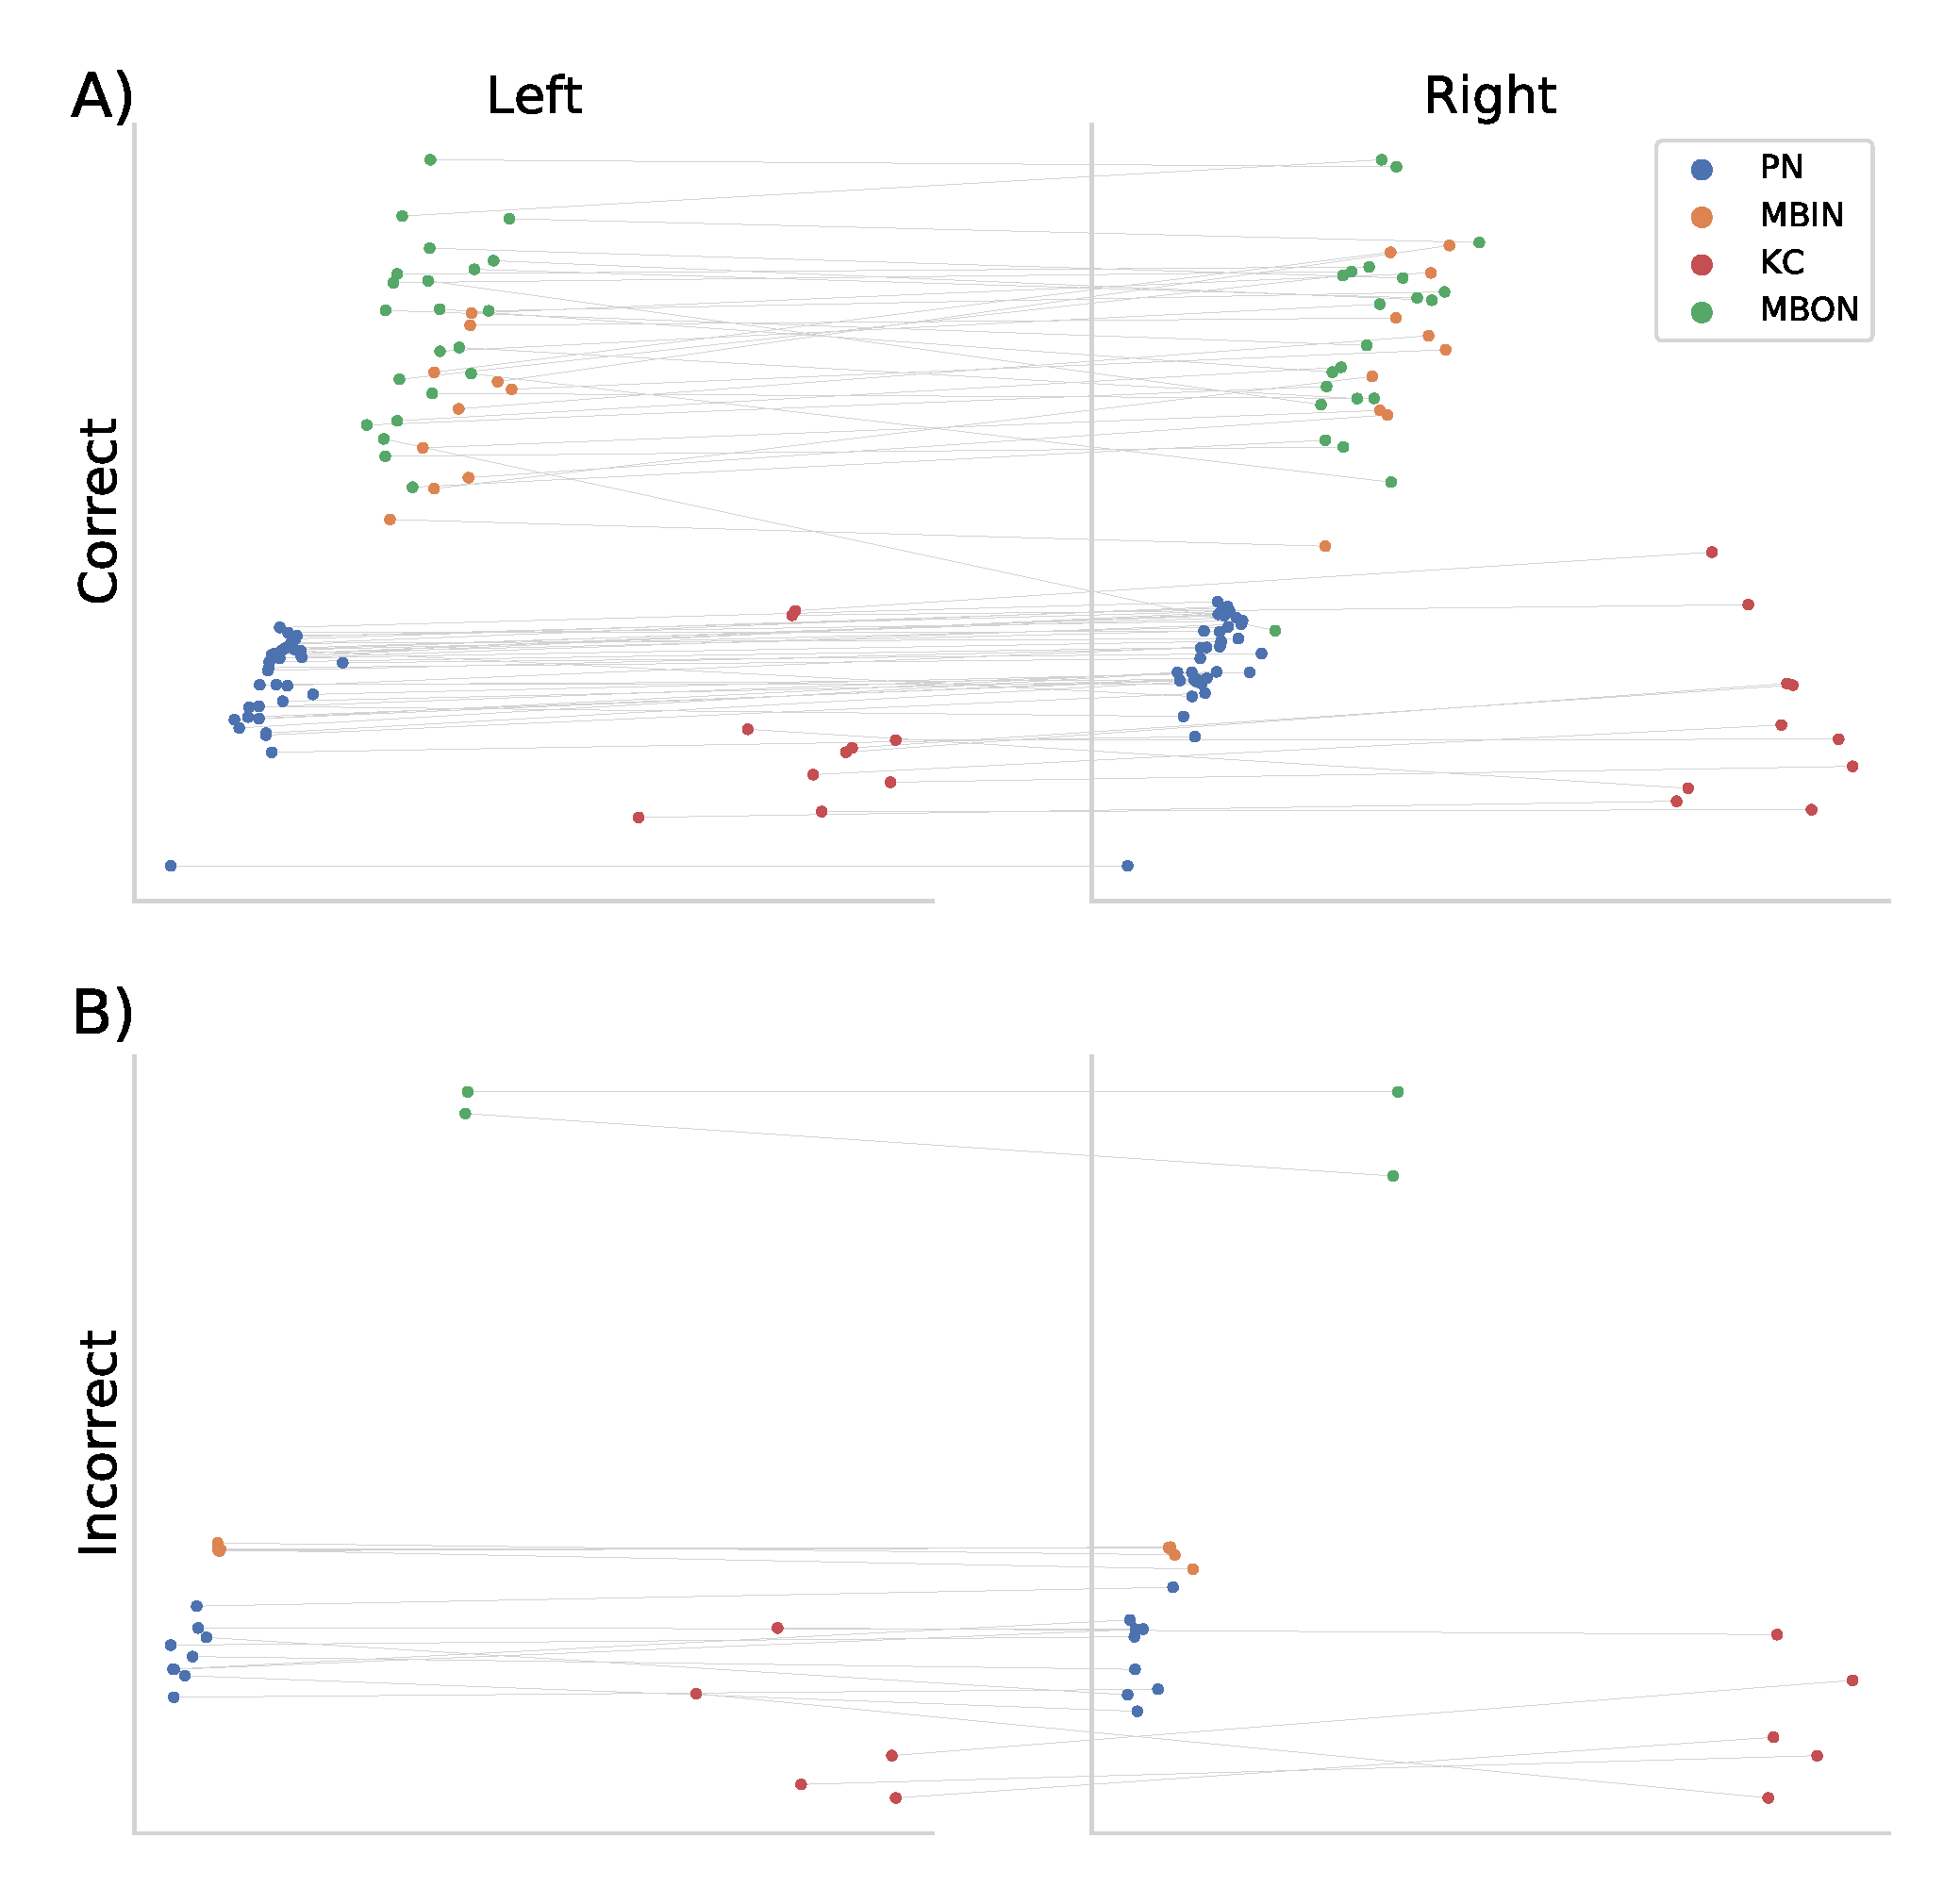
\includegraphics[width = .8\linewidth]{figures/dnd/mb-matching.pdf}
    \caption
    [Graph matching on the \textit{Drosophila} mushroom body network.]
    {\textbf{Graph matching on the \textit{Drosophila} mushroom body network.} All panels show the first two dimensions of principal component analysis $\mathtt{PCA}$ on the adjacency spectral embedding ($\ase$) of the mushroom body network (for visualization purposes). Each point represents a neuron in the network which has a manually identified pair in the opposite hemisphere, and colors represent one of Kenyon cells, input neurons, output neurons, and projection neurons. 
    Lines show the neuron pair that was predicted by graph matching. 
    \textbf{a.} All of the correctly matched neuron pairs. 78.8\% of neuron pairs (78/99) were correctly matched. 
    \textbf{b.} All of the incorrectly matched neuron pairs. Note that all of the incorrectly matched neurons are matched to neurons of the same cell type.}
    \label{fig:mb-matching}
\end{figure}

\subsection{Testing for Significant Edges} \label{sec:exp1}
We consider two populations of networks generated from an $\er$ model and a 2-block $\mathsf{Kidney-Egg}~\sbm$ model. All networks have $n=20$ vertices and $\pi = \bracks*{0.25, 0.75}$. The block probability matrices for each population is given by $\B^{(1)} = [p, p; p, p]$ and $\B^{(2)} = [p+\delta, p; p, p]$ where $p=0.5$. 
The difference between the two population is in the first block, $\B_{11}$, and $\delta$ is the magnitude of the difference which ranges from $0$ to $(1-p)$. In other words, $\delta$ is the effect size. Total of $m$ networks are sampled ($\frac{m}{2}$ networks per population). 
For each edge, the t-test test statistics is computed between the two populations, which are then ranked from largest to smallest in magnitude. Ranking of the test statistics and a cutoff is utilized rather than p-value corrections (e.g. Bonferroni) to control for false positive rate. In this case, the ten edges with largest magnitudes are considered since we expect ten edges to be different. 
Non-parametric tests are not considered since many of them are based on ranking the underlying data, which is not sensible for binary data. 
The performance is evaluated with recall@10, which quantifies the fraction of the top ten ranked edges are indeed the truly different edges, averaged over 100 repeated trials.

Figure \ref{fig:exp1}a shows that when the effect size is small ($\delta \leq 0.05$), significant edges cannot be detected even at largest sample sizes ($m=1000$). On the other hand, when effect size is large ($\delta \geq 0.45$), significant edges can be perfectly detected at relatively small sample sizes ($m \geq 30$). 

Connectivity in human brains was analyzed using the structural connectomes (see Appendix \ref{sec:hcp}). For each edge, the class conditional mean, which is the estimated connectivity probability, is computed for females ($m = 572$) and males ($m=488$). The sample sizes and difference in conditional means, which is the estimated effect size, are used to find the closest recall@10 values from the simulated experiment, denoted empirical trustworthiness shown in Figure \ref{fig:exp1})b. Thus, empirical trustworthiness is the confidence in which one can trust that a significant edge is truly significant. There are 2380 possible total edges in connectomes with 70 vertices, but only 49 edges have trustworthiness $\geq 0.9$, meaning one can only trust significance for small set of edges.

\begin{figure}
    \centering
    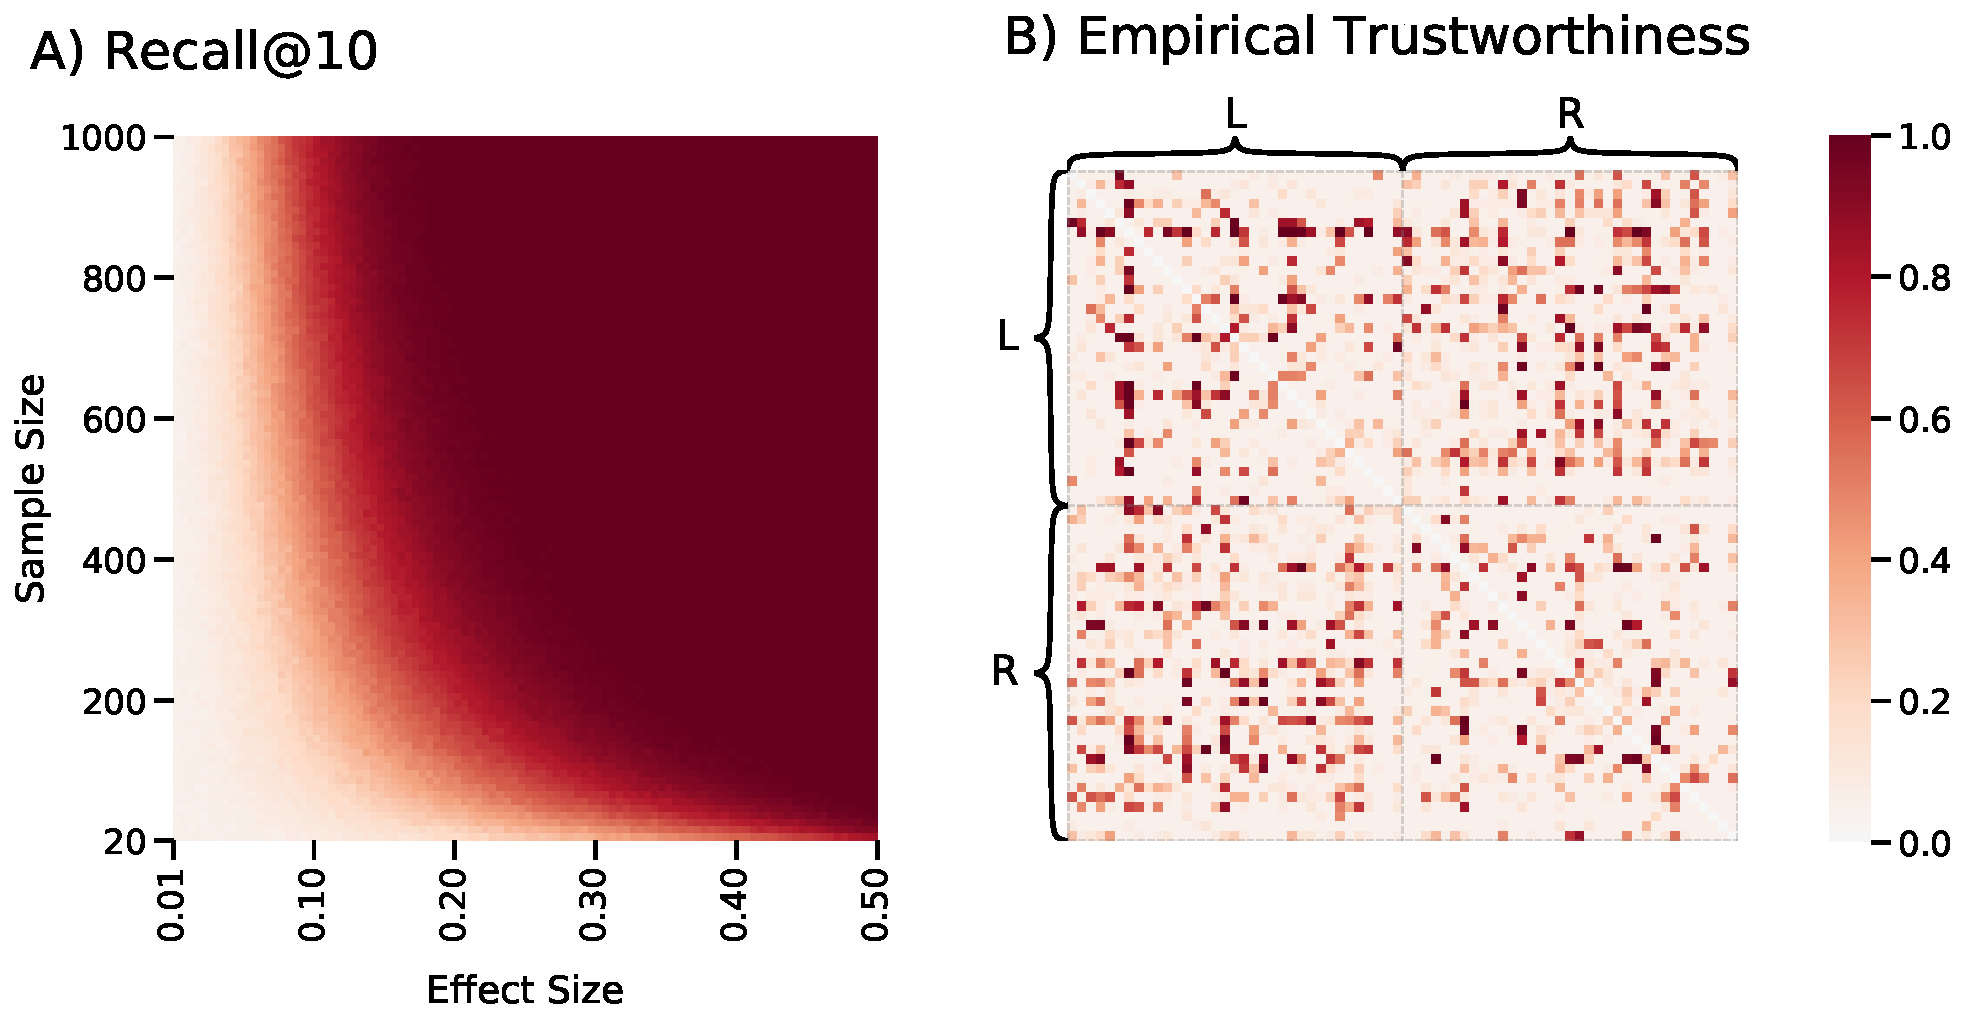
\includegraphics[width=.75\textwidth]{figures/dnd/exp1_final}
    \caption
    [Performance of finding significant edges in two different populations of networks.]
    {\textbf{Performance of finding significant edges in two different populations of networks.}
    \textbf{a.} Recall for varying sample size and effect size when comparing two populations of binary networks using t-test.
    The color bar represents recall@10 averaged over 100 trials. 
    When effect size is small, significant edges cannot be detected even at large sample size. When effect size is large, significant edges can be detected at small sample sizes ($m=1000$). 
    \textbf{b.} Analysis of structural connectomes from the Human Connectome Project (HCP) data, and the vertices are organized by left (L) and right (R) hemispheres. Edge weights are binarized to parallel the simulations. Heatmap shows the empirical trustworthiness of significant edges when comparing each edge between females and males.}
    \label{fig:exp1}
\end{figure}

Appendix \ref{sec:exp3} investigates the edge-wise testing in weighted connectomes. We leverage the t-test, Mann-Whitney, and Kolmogorov-Smirnov (KS) test, which is a non-parametric test of whether there exists a difference in empirical cumulative distributions between edge weights. We find that KS test is the only test that is appropriate for weighted edges since KS test can detect changes in not only the means, but also changes in variance. In weighted HCP connectomes, we find that 256 edges have trustworthiness $\geq 0.9$, and that very small fraction of edges can be trusted to be significant.

\subsection{Testing for Significant Vertices}

\begin{figure} 
    \centering
    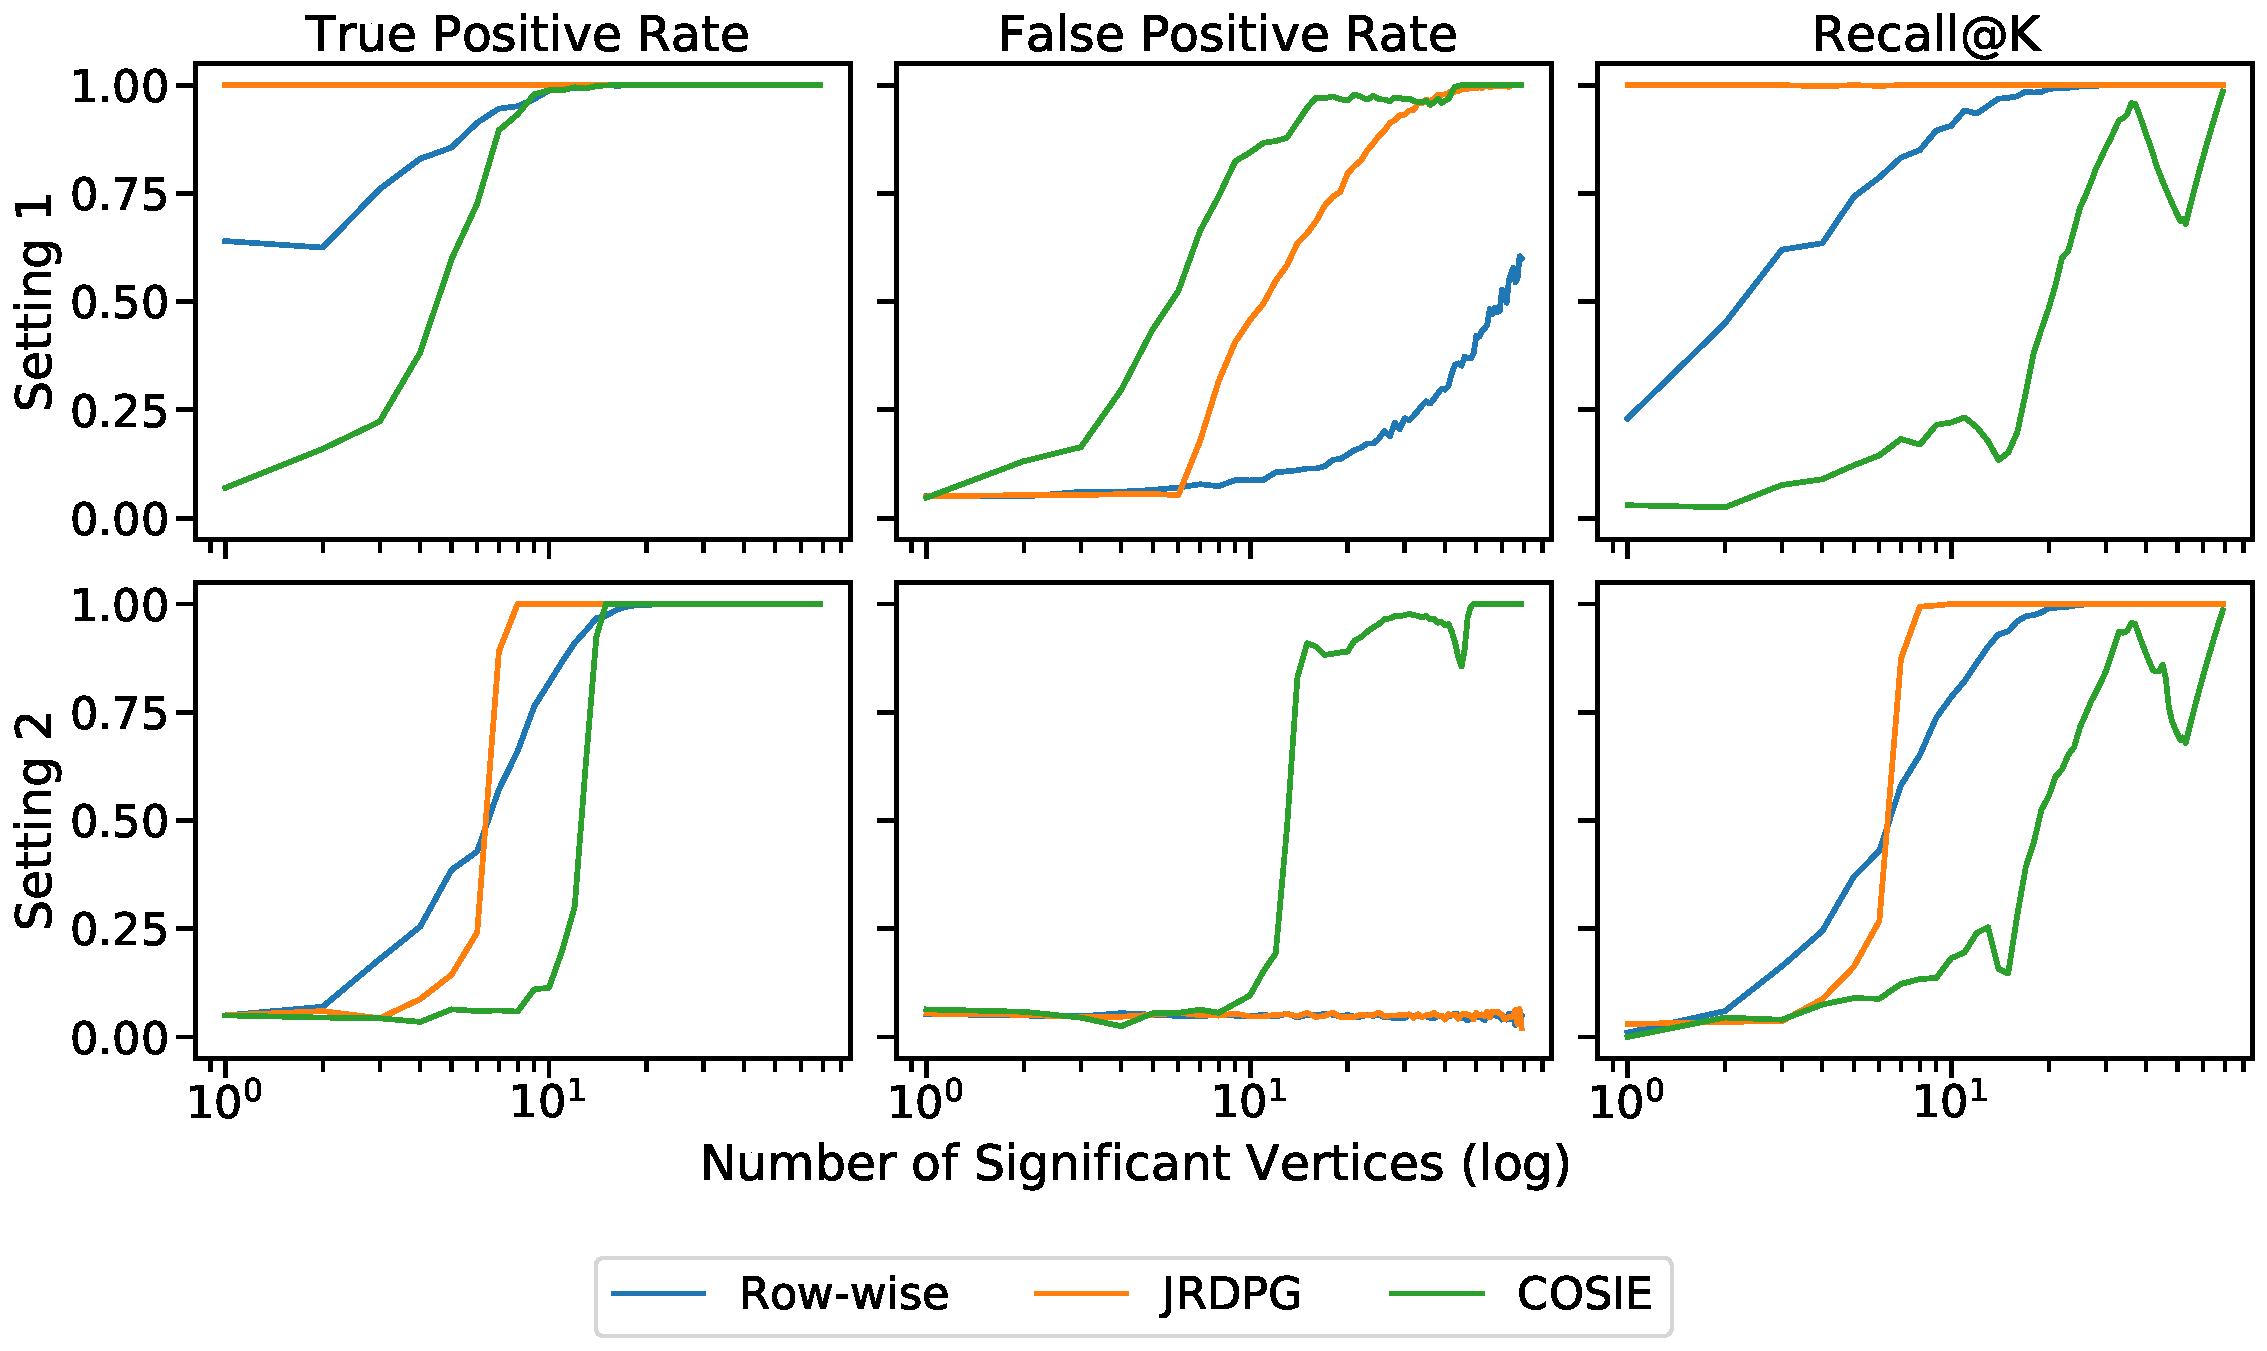
\includegraphics[width=.8\textwidth]{figures/dnd/exp7_new}
    \caption
    [Performance for finding significant vertices using various representations of vertices.]
    {\textbf{Performance for finding significant vertices using various representations of vertices.} We compare a population of graphs from a planted partition stochastic block model ($\sbm$) and another from a symmetric heterogeneous $\sbm$ in two different settings. The number of vertices for each graph is kept constant ($n=70$), but the number of significantly different vertices is varied (x-axis). \textit{(Top row)} In this setting, all three representations are not valid as the false positive rate increases with the number of significant vertices. \textit{(Bottom row)} In this setting, row-wise and joint random dot product graphs ($\jrdpg$) representations are valid while common subspace independent-edge model ($\cosie$) representation is not. 
    In both settings, the sorting of the p-values can be trusted as recall@$K$ increases as number of significant vertices increase.
    }
    \label{fig:exp7}
\end{figure} 

In this section, we test for significant vertices using different representations of vertices. 
Simplest representation is a set of edges, where the corresponding row (or column) of a vertex in the adjacency matrices are collected and tested for difference. 
Another is the low-dimensional latent-space representation using the $\jrdpg$ and $\cosie$ models, and the latent positions of vertices are tested for difference. Since all representations are multivariate, hypothesis are tested using Hotelling's test, which is a multivariate generalization of t-test.

We consider a population of planted partition $\sbm$ and a symmetric heterogeneous $\sbm$ in two different settings. In both settings, the planted partition $\sbm$ has $\B^{(1)} = [0.125, 0.0625; 0.0625, 0.125]$ block probability matrix. In setting 1, the symmetric heterogeneous $\sbm$ has  $\B^{(2)} = [0.125, 0.088; 0.088, 0.25]$ block probability matrix, and in setting 2, $\B^{(2)} = [0.125,  0.0625; 0.0625, 0.25]$. The vertices that belong to the second block, which has the different within-block probability, are considered significant vertices, and we vary the number of vertices that belong to the second block. Total of $m=100$ networks are sampled per population, and the p-values are computed using Hotelling's on each of the three vertex representations for each vertex. Vertices with p-values less than $\alpha=0.05$ after Bonferroni correction are considered significant. The performance is measured via true positive rate (TPR), false positive rate (FPR), and recall@$K$, where $K$ is the number of significant vertices. 

Figure \ref{fig:exp7} shows that the $p$-values cannot necessarily be trusted. That is, in some settings, the significant vertices cannot be trusted due to uncontrolled FPR. However, the sorting of $p$-values can be trusted in both settings. Thus, in situations when the underlying model is not known (i.e. in real data), one should trust the sorting of the $p$-values (or test statistic), but not the magnitudes. 
